\section{Introduction}

Robots are frequently used in remote and unpredictable environments.
%
% One trouble of using robots in these environments is that they must be capable of navigating highly varied terrain.
%
For example, in \emph{search and rescue} robots are designed to aid first responders search for victims in hazordous and highly varied terrain~\citep{Graf.2017.2ISSCIS.RescuePathOptimization}.
%
One solution to this problem is to use an unmanned aerial vehicle (UAV). However, UAVs can typically only operate for short periods of time (roughly 30 minutes to one hour).

More recently, lightweight mobile robots with transformable wheels have been developed for search and rescue.
%
As shown in Figure~\ref{fig:robot}, a transformable wheel robot is capable of extending struts radially outward from the center of each wheel. These struts help the robot climb over obstacles that are roughly the same size as the robot~\citep{Clark.2018.C.EvolvingControllersTransformable}.
%
These devices have the benefits of normal wheels (e.g., increased stability and less vibration) and legged-wheels (e.g., increased mobility), and they have a longer operating duration compared to UAVs.


\begin{figure}[!ht]
    \centering

    \subfloat[Physical Simulation]{%
        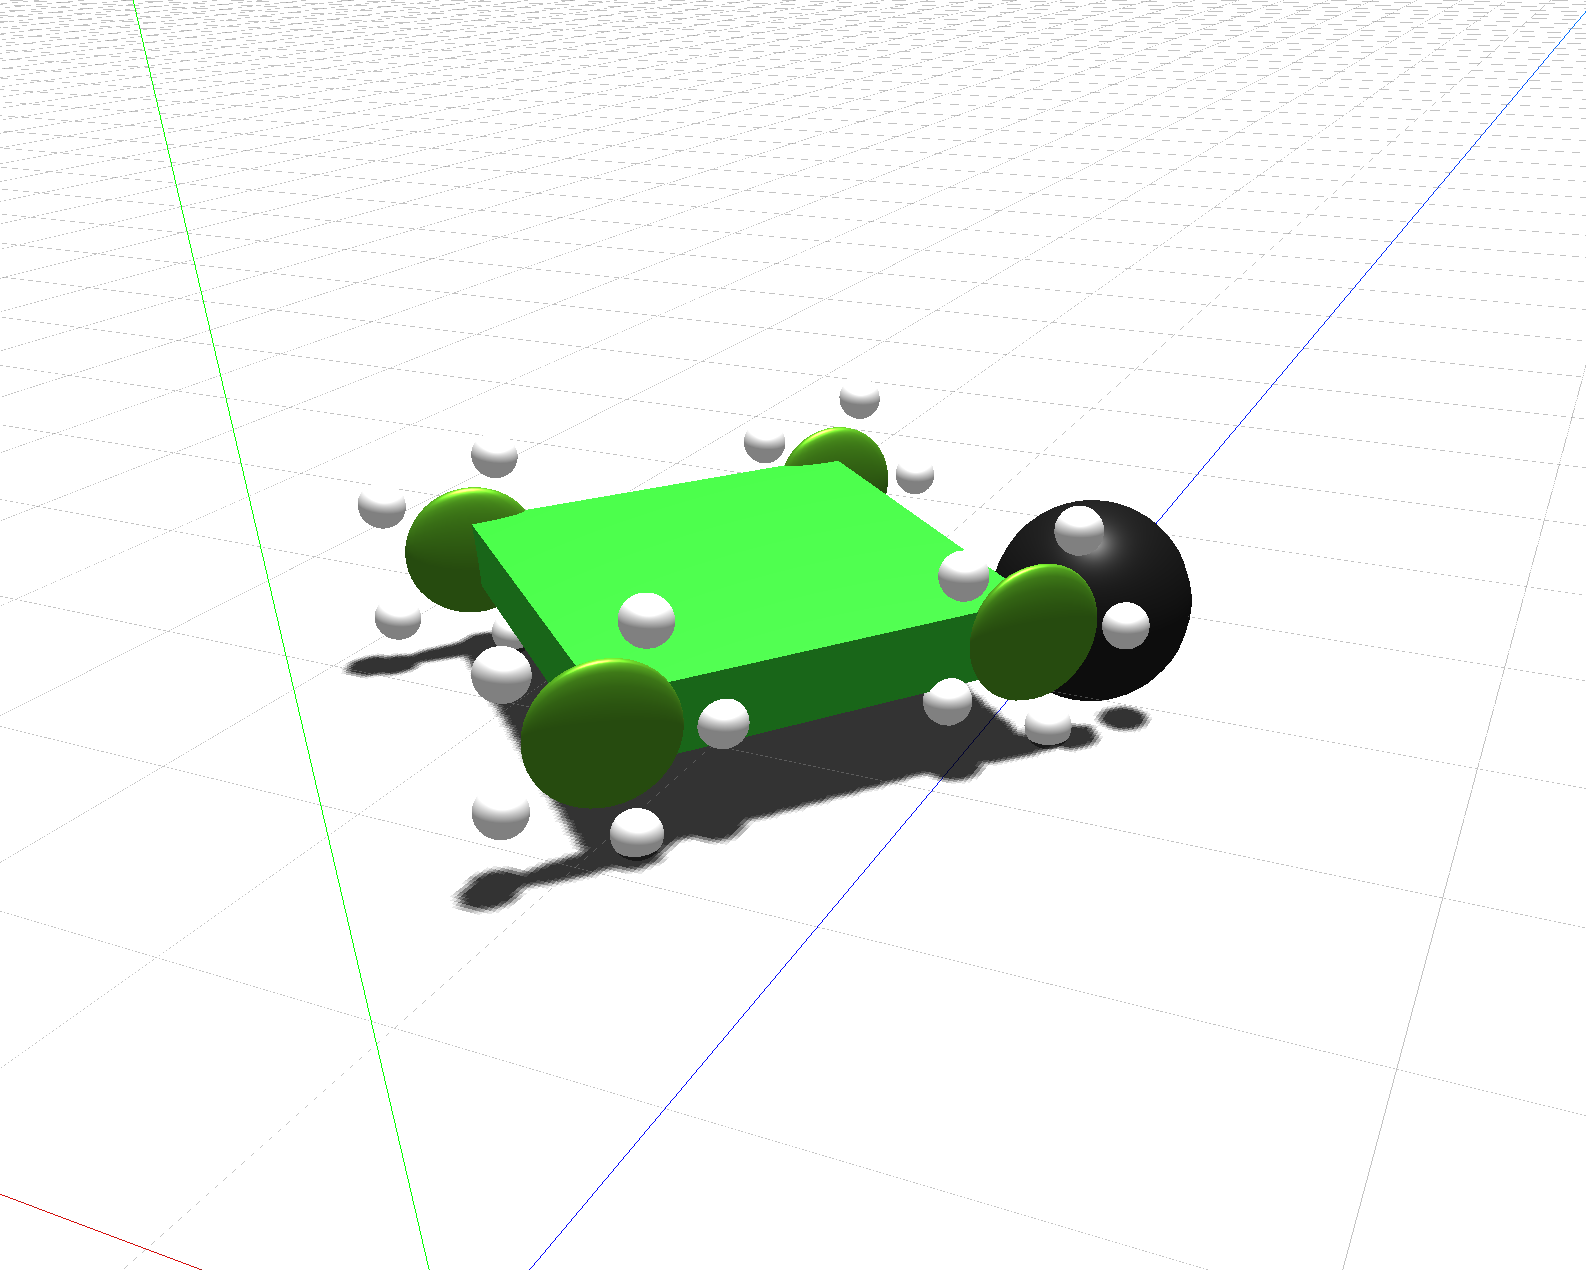
\includegraphics[width=0.4\columnwidth,valign=c]{figures/physical-simulation.png}%
        \vphantom{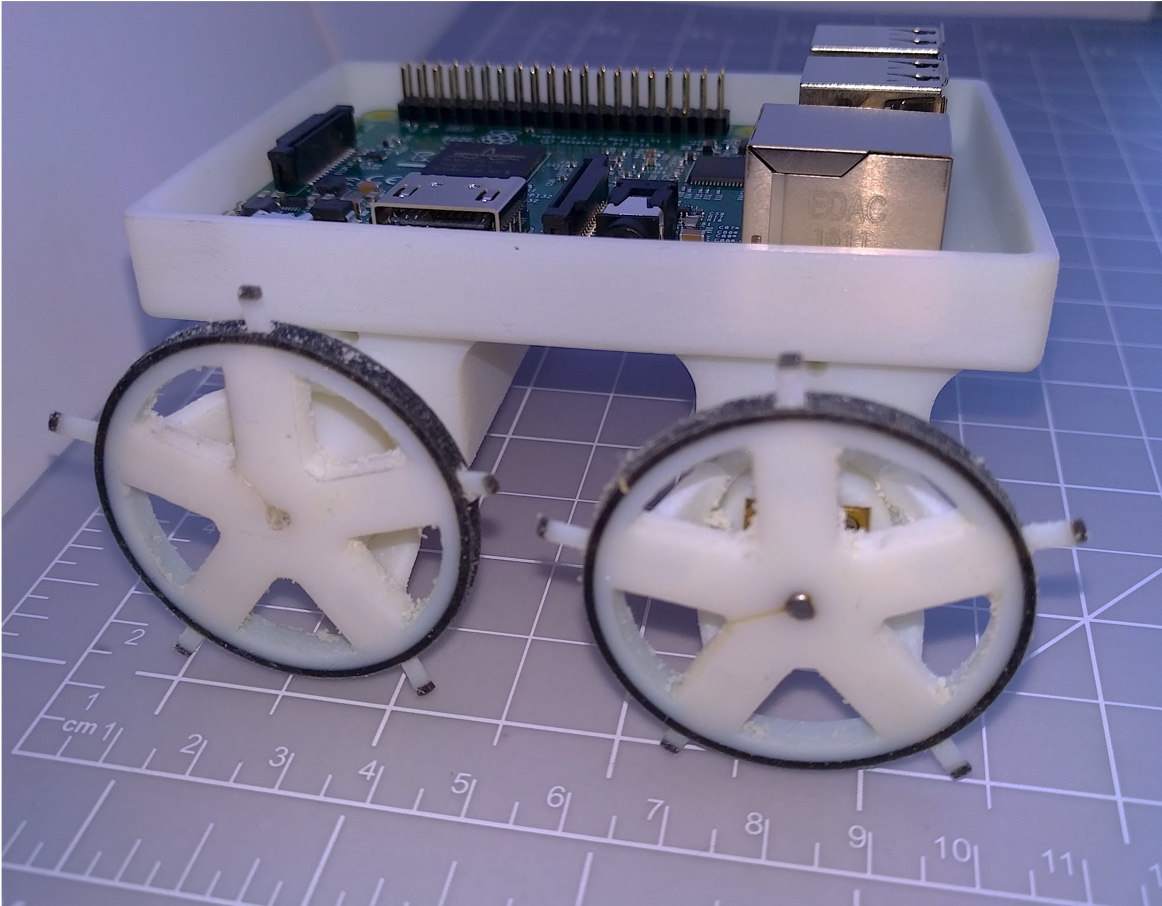
\includegraphics[width=0.4\columnwidth,valign=c]{figures/perspective-image.jpg}}%
    }\quad
    \subfloat[Prototype]{%
        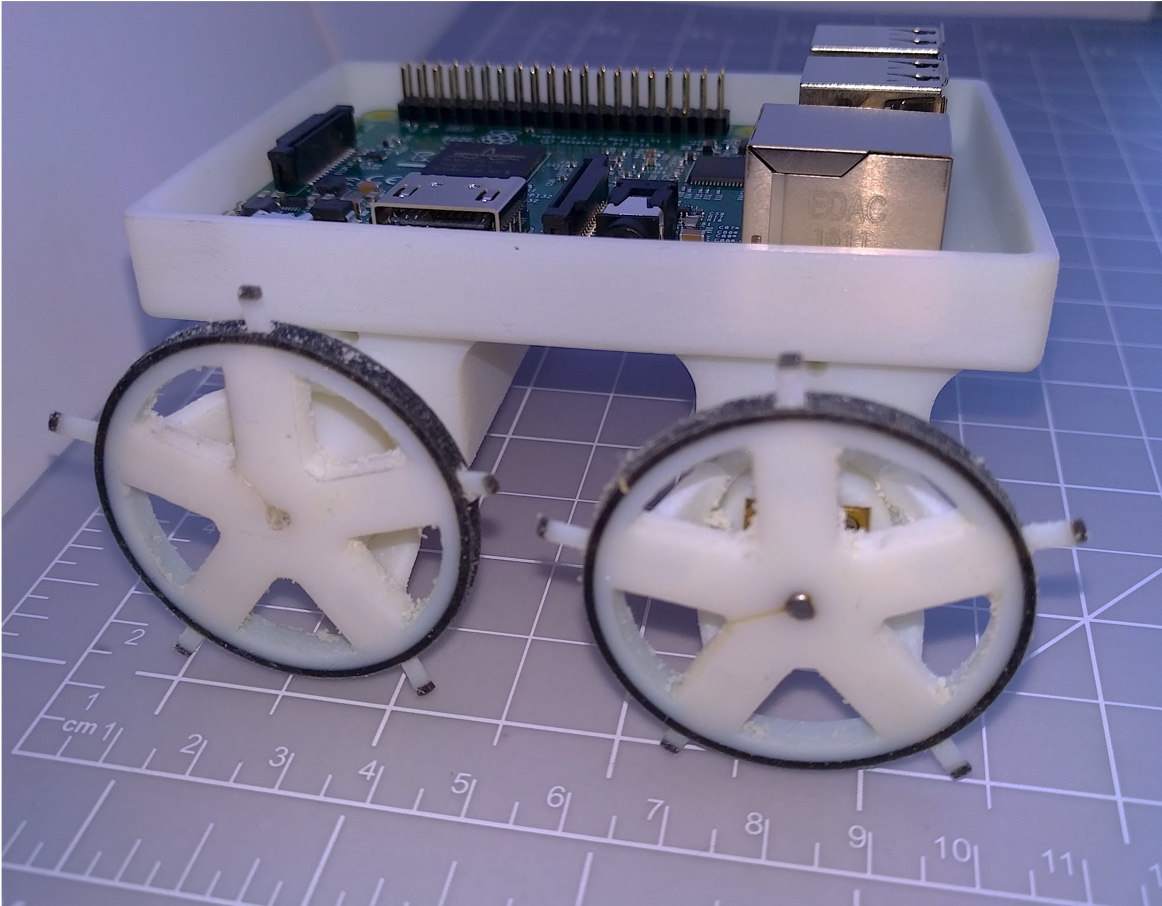
\includegraphics[width=0.4\columnwidth,valign=c]{figures/perspective-image.jpg}%
    }

    \vspace{-0.1in}

    \caption{A mobile robot with transformable wheels.}
    \label{fig:robot}

    \vspace{-0.45in}

\end{figure}

A drawback of using a transformable wheel mobile robot (or a legged-wheel robot) is that they are difficult to model.
%
Without an accurate model of the robot, it is difficult to determine when wheels should transform from normal wheels into legged-wheels.
%
Specifically, a model can calculate the \emph{expected} velocity of the robot, and we can compare this quantity to the \emph{real} velocity as measured by sensors. If these two quantities differ by some threshold amount, then the robot should infer that it is stuck or slipping (i.e., it is exhibiting poor mobility) and it should extend its wheel struts.
%
Without an accurate model of the robot kinematics, this process cannot work.


\begin{figure*}[ht]
    \centering
    \subfloat[]{%
        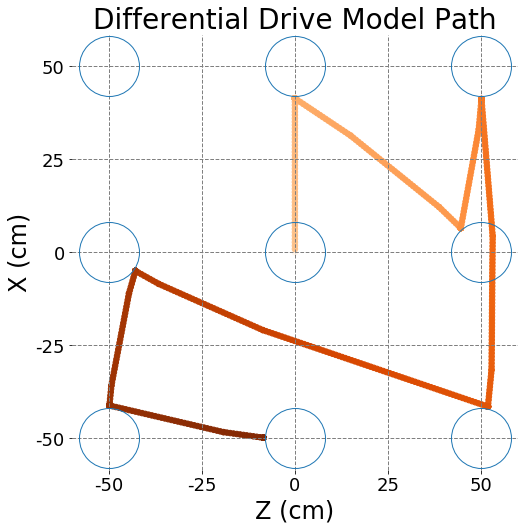
\includegraphics[height=1.6in]{figures/ddm-path.png}%
    }\hfil
    \subfloat[]{%
        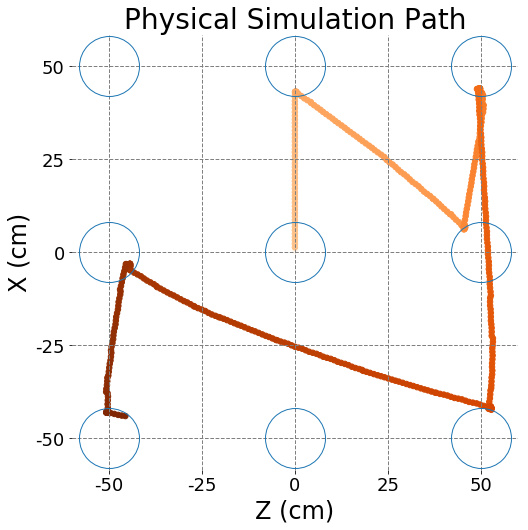
\includegraphics[height=1.6in]{figures/phy-path.png}%
    }\hfil
    \subfloat[]{%
        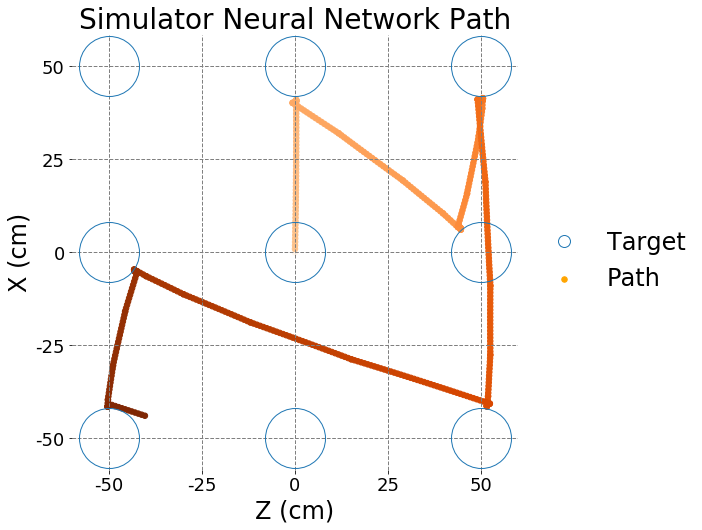
\includegraphics[height=1.6in]{figures/snn-path.png}%
    }
    %\vspace{-0.05in}
    \caption{Example paths taken by the robot (a) as predicted by the differential drive model, (b) during a physical simulation, and (c) as predicted by a trained SNN. Blue circles represent way-points that the robot is trying to reach in a pre-defined sequence. The robot moves on to its next way-point once it reaches to within 10\si{cm} of its current target way-point. Robot paths are shown in orange, and lighter shades denote earlier an earlier time in simulation (the robot starts at the origin).}
    \label{fig:paths}
    %\vspace{-0.15in}
\end{figure*}

\noindent
\textbf{Related work.}
%
In prior work, we use a differential drive model to calculate \emph{expected} velocity~\citep{Clark.2018.C.EvolvingControllersTransformable}. This process was error prone.
%
The model did not account for strut extension, wheel slippage (i.e., differing friction properties of different terrains), uneven ground, or that the wheels might rotate at a different rate than commanded.
%
In this study, we develop a simulator neural network (SNN) similar to that described by \citet{Pretorius.2014.2ICECC.ComparisonNeuralNetworks}, where they train a neural network so that control signals map to changes the pose of the robot.
%
The goal of this study is to produce an accurate model of our mobile robot. The model will have two uses: (1) to act in place of a physical simulation for optimizing control parameters and (2) to determine when the robot exhibits poor mobility and should extend struts.
